%% FEI-template.tex
%% Este trabalho utiliza uma adaptação da classe USPSC.cls que é mantida pela seguinte equipe:
%% 
%% Coordenação e Programação:
%%   - Marilza Aparecida Rodrigues Tognetti - marilza@sc.usp.br (PUSP-SC)
%%   - Ana Paula Aparecida Calabrez - aninha@sc.usp.br (PUSP-SC)
%% Normalização:
%%   - Brianda de Oliveira Ordonho Sigolo - brianda@usp.br (IAU)
%%   - Eduardo Graziosi Silva - edu.gs@sc.usp.br (EESC)
%%   - Eliana de Cássia Aquareli Cordeiro - eliana@iqsc.usp.br (IQSC)
%%   - Flávia Helena Cassin - cassinp@sc.usp.br (EESC)
%%   - Maria Cristina Cavarette Dziabas - mcdziaba@ifsc.usp.br (IFSC)
%%   - Regina Célia Vidal Medeiros - rcvmat@icmc.usp.br (ICMC)
%%



%----------------------------------------------------------------
%% Sobre a classe abntex2.cls:
%% abntex2.cls, v-1.9.5 laurocesar
%% Copyright 2012-2015 by abnTeX2 group at https://www.abntex.net.br/ 
%%
%----------------------------------------------------------------

\documentclass[
% -- opções da classe memoir --
12pt,		% tamanho da fonte
%openright,	% capítulos começam em pág ímpar (insere página vazia caso preciso)
oneside,  % para impressão em anverso (frente) e verso. Oposto a oneside - Nota: utilizar \imprimirfolhaderosto*
%oneside, % para impressão em páginas separadas (somente anverso) -  Nota: utilizar \imprimirfolhaderosto
% inclua uma % antes do comando twoside e exclua a % antes do oneside 
a4paper,			% tamanho do papel. 
% -- opções da classe abntex2 --
chapter=TITLE,		% títulos de capítulos convertidos em letras maiúsculas
% -- opções do pacote babel --
english,			% idioma adicional para hifenização
french,				% idioma adicional para hifenização
spanish,			% idioma adicional para hifenização
brazil				% o último idioma é o principal do documento
]{classe/USPSC}

% ---
% Pacotes básicos - Fundamentais 
% ---
\usepackage[T1]{fontenc}		% Seleção de códigos de fonte.
\usepackage[utf8]{inputenc}		% Codificação do documento (conversão automática dos acentos)
\usepackage{times}		    	% Usa a fonte Times New Roman							
\usepackage{lastpage}			% Usado pela Ficha catalográfica
\usepackage{indentfirst}		% Indenta o primeiro parágrafo de cada seção.
\usepackage{color}				% Controle das cores
\usepackage{graphicx}			% Inclusão de gráficos
\usepackage{float} 				% Fixa tabelas e figuras no local exato
\usepackage{chemfig}            % Para escrever reações químicas
\usepackage{chemmacros}         % Para escrever reações químicas
\usepackage{tikz}				% Para escrever reações químicas e outros
\usetikzlibrary{positioning}
\usepackage{microtype} 			% para melhorias de justificação
\usepackage{pdfpages}
\usepackage{makeidx}            % para gerar índice remissivo
\usepackage{hyphenat}          % Pacote para retirar a hifenizacao do texto
\usepackage[absolute]{textpos} % Pacote permite o posicionamento do texto
\usepackage{eso-pic}           % Pacote para incluir imagem de fundo
\usepackage{makebox}           % Pacote para criar caixa de texto
\usepackage{setspace}
\usepackage{caption}
\captionsetup[table]{justification=raggedright, singlelinecheck=false, width=\textwidth} % Alinha a legenda da tabela à esquerda
\captionsetup[quadro]{justification=raggedright, singlelinecheck=false, width=\textwidth} % Alinha a legenda da tabela à esquerda	
\captionsetup[figure]{justification=raggedright, singlelinecheck=false, width=\textwidth} % Alinha a legenda da tabela à esquerda	
% ---
% Pacotes de citações
% Citações padrão ABNT
% ---
% Sistemas de chamada: autor-data ou numérico.
% Sistema autor-data
\usepackage[alf, abnt-emphasize=bf, abnt-thesis-year=both, abnt-repeated-author-omit=no, abnt-last-names=abnt, abnt-etal-cite=3, abnt-etal-list=3, abnt-etal-text=it, abnt-and-type=e, abnt-doi=doi, abnt-url-package=none, abnt-verbatim-entry=no]{abntex2cite}
\bibliographystyle{classe/abntex2-alf-USPSC}


% Se o idioma for o inglês, inclua % no comando acima e exclua o % do comando abaixo
%\bibliographystyle{USPSC-classe/abntex2-alfeng-USPSC}


% Complementarmente, verifique as instruções abaixo sobre os Pacotes de Nota de rodapé
% ---
% Pacotes de Nota de rodapé
% Configurações de nota de rodapé


\renewcommand{\footnotesize}{\small} %Comando para diminuir a fonte das notas de rodapé
\renewcommand{\ABNTEXchapterfont}{\rmfamily}
\newcommand{\citefonte}[1]{\fontsize{10}{12}\selectfont\citeauthor{#1}, \citeyear{#1}} %Exibe como Autor,Ano em fonte 10 para Fontes de Tabelas, Quadros e Figuras


% ---
% Pacotes adicionais, usados apenas no âmbito do Modelo Canônico do abnteX2
% ---
\usepackage{lipsum}				% para geração de dummy text
% ---

% pacotes de tabelas
\usepackage{multicol}	% Suporte a mesclagens em colunas
\usepackage{multirow}	% Suporte a mesclagens em linhas
\usepackage{longtable}	% Tabelas com várias páginas
\usepackage{threeparttablex}    % notas no longtable
\usepackage{array}


% Pacotes para Overleaf
%\usepackage{showframe} % Para resolver "Underfull \hbox" e "Underfull \vbox"

% ----
% Compatibilização com a ABNT NBR 6023:2018 e 10520:2023
\usepackage{classe/ABNT6023-10520}



% Os demais dados deverão ser fornecidos no arquivo FEI-pre-textual
% Configurações de aparência do PDF final
% alterando o aspecto da cor azul
\definecolor{blue}{RGB}{41,5,195}

% informações do PDF
\makeatletter
\hypersetup{
	pdftitle={xxxx}, 
	pdfauthor={lwila},
	pdfsubject={\imprimirpreambulo},
	pdfcreator={LaTeX with abnTeX2},
	colorlinks=true,       		% false: boxed links; true: colored links
	linkcolor=black,          	% color of internal links
	citecolor=black,        		% color of links to bibliography
	filecolor=black,      		% color of file links
	urlcolor=black,
	%Para habilitar as cores dos links, retire a % antes dos comandos abaixo e inclua a % antes das 4 linhas de comando acima 
	%linkcolor=blue,            	% color of internal links
	%citecolor=blue,        		% color of links to bibliography
	%filecolor=magenta,      		% color of file links
	%urlcolor=blue,
	bookmarksdepth=4	
}
\makeatother
% --- 

% O tamanho do parágrafo é dado por:
\setlength{\parindent}{1.3cm}

% ---
% compila o sumário e índice
\makeindex
% ---

% ----
% Início do documento
% ----
\begin{document}

% Seleciona o idioma do documento (conforme pacotes do babel)
\selectlanguage{brazil}
% Se o idioma do texto for inglês, inclua uma % antes do 
%      comando \selectlanguage{brazil} e 
%      retire a % antes do comando abaixo
%\selectlanguage{english}

% Retira espaço extra obsoleto entre as frases.
\frenchspacing 

% --- Formatação dos Títulos
\renewcommand{\ABNTEXchapterfontsize}{\fontsize{12}{12}\bfseries}
\renewcommand{\ABNTEXsectionfontsize}{\fontsize{12}{12}\normalfont}
\renewcommand{\ABNTEXsubsectionfontsize}{\fontsize{12}{12}\bfseries}
\renewcommand{\ABNTEXsubsubsectionfontsize}{\fontsize{12}{12}\bfseries\itshape}
\renewcommand{\ABNTEXsubsubsubsectionfontsize}{\fontsize{12}{12}\normalfont}

% ----------------------------------------------------------
% ELEMENTOS PRÉ-TEXTUAIS
% ----------------------------------------------------------
% ---
% Capa
% ---
\imprimircapa
% ---
% Folha de rosto
% (o * indica impressão em anverso (frente) e verso )
% ---
\imprimirfolhaderosto*
%\imprimirfolhaderosto
% ---
% ---
% Inserir a ficha catalográfica em pdf
% ---
% A biblioteca da sua Unidade lhe fornecerá um PDF com a ficha catalográfica definitiva. 
% Quando estiver com o documento, salve-o como PDF no diretório 
% do seu projeto como fichacatalografica.pdf e inclua o arquivo 
% utilizando o comando abaixo:
 
%\includepdf{PreTextual/fichacatalografica.pdf}

% Se você optar por elaborar a ficha catalográfica, deverá 
%  retirar o % do comando abaixo
%% USPSC-fichacatalografica.tex
% ---
% Inserir a ficha bibliografica
% ---

\begin{center}
\large{A ficha catalográfica deve ser gerada automaticamente neste link: 
\url{https://ficha.fei.edu.br/ficha/?_gl=1*1wyaveq*_gcl_au*MTY2MDUzNTY0OC4xNzMwMjI1MzEw*_ga*MTc3NDA5MjgwOC4xNzIyNDQ3NzE5*_ga_9CWNLCJN1W*MTczMjg5ODUxNC40NjcuMS4xNzMyODk4NTE2LjU4LjAuMA}}
\end{center}

% As informações que compõem a ficha catalográfica estão 

% ---
% Inserir folha de aprovação
% ---

% A Folha de aprovação é um elemento obrigatório da NBR 4724/2011 (seção 4.2.1.3). 
% Após a defesa/aprovação do trabalho, gere o arquivo folhadeaprovacao.pdf da página assinada pela banca pelo Ábaris
% e iclua o arquivo utilizando o comando abaixo:
%\includepdf{PreTextual/folhadeaprovacao.pdf}

% Alternativa para a Folha de Aprovação:
% Se for a sua opção elaborar uma folha de aprovação, insira uma % antes do comando acima que inclui o arquivo folhadeaprovacao.pdf,
% tire o % do comando abaixo e altere o arquivo folhadeaprovacao.tex conforme suas necessidades
%% USPSC-folhadeaprovacao.tex
% Alternativa para a Folha de Aprovação 
% Se esta for a sua opção, exclua inclusão feita acima do arquivo folhadeaprovacao.pdf
%
\begin{folhadeaprovacao}
  \begin{center}
       {\ABNTEXchapterfont\normalfont\imprimirautor}\\
\textbf{PARA PÓS-GRADUAÇÃO, SUBSTITUIR ESSA  FOLHA DE APROVAÇÃO  PELA FOLHA ATA}
	 \vspace*{2cm}
   
    \begin{center}
      \ABNTEXchapterfont\bfseries\MakeUppercase\imprimirtitulo

    \end{center}
		\vspace*{3cm}
		\hspace{.45\textwidth}
    \begin{minipage}{.5\textwidth}
        \imprimirpreambulo
    \end{minipage}
		\vspace*{2cm}
    %\vspace*{\fill}
	\end{center}

  \begin{center}
		
	  {\ABNTEXchapterfont\normalfont\ {Comiss\~ao Julgadora:} \\}
		%Trabalho aprovado. \imprimirlocal, 2 de outubro de 2015:
		
		%\assinatura{\textbf{\imprimirorientador} \\ Orientador} 
		%\assinatura{\textbf{\imprimirorientador} \\}
    % Se for ORIENTADOR, inclua % no início do comando abaixo e tire a % do próximo comando 
		%\renewcommand{\orientadorname}{Orientadora}
		%\renewcommand{\orientadorname}{Orientador}

		\assinatura{Nome Orientador}
		
		\assinatura{Professor 1}
		
		\assinatura{Professor 2}
		%\assinatura{\textbf{Professor} \\ Convidado3}
		%\assinatura{\textbf{Professor} \\ Convidado4}
		%\begin{center}
		\vspace*{4cm}
   	{\ABNTEXchapterfont\normalfont\imprimirlocal}
    \par
%Adicionar data de aprovação da Banca
  {\ABNTEXchapterfont\normalfont\ {02 de outubro de XXXX} \\}
\end{center}
\end{folhadeaprovacao}
% ---

% ---
% Dedicatória
% ---
%% USPSC-Dedicatoria.tex
\begin{dedicatoria}
 \vspace*{20cm}
\noindent\hspace{8cm} % Recuo de 8 cm à esquerda
\begin{minipage}{8cm} % Define a largura do texto
    {\setlength{\baselineskip}{1.5\baselineskip} % Espaçamento de 1,5 entre linhas
    \noindent % Garantir alinhamento inicial
    {Espaço reservado para a dedicatória,justificado com 8cm de recuo à esquerda, com espaçamento entre linhas 1,5.}}
\end{minipage}

\end{dedicatoria}
% ---
% ---

% ---
% Agradecimentos
% ---
%% USPSC-Agradecimentos.tex

\begin{agradecimentos}
\vspace{-\baselineskip} %Manter para garantir o espaçamento da biblioteca.
Espaço reservado para os agradecimentos. Iniciado com parágrafo de 1,25. Espaçamento entre linhas 1,5.
\end{agradecimentos}
% ---
% ---

% ---
% Epígrafe
% ---
%% USPSC-Epigrafe.tex
\begin{epigrafe}
 \vspace*{20cm}
\noindent\hspace{8cm} % Recuo de 8 cm à esquerda
\begin{minipage}{8cm} % Define a largura do texto
    {\setlength{\baselineskip}{1.5\baselineskip} % Espaçamento de 1,5 entre linhas
    \noindent % Garantir alinhamento inicial
    {Espaço reservado para a epígrafe (apresentar entre aspas, digitada em espaço 1, 5 entre linhas, 8 cm de recuo à esquerda e justificada.  Acrescentar na lista de referências).}}
\end{minipage}
\end{epigrafe}
% ---
% ---

% A T E N Ç Ã O
% Se o idioma do texto for em inglês, o abstract deve preceder o resumo
% resumo em português
%
% Resumo
% ---
%% USPSC-Resumo.tex

\begin{resumo}
\setlength{\baselineskip}{1.5\baselineskip} % Espaçamento de 1,5 entre linhas

Elaborado pelo próprio autor, apresentação concisa dos pontos relevantes de um documento. Deve ressaltar o objetivo, o método, os resultados e as conclusões do documento. O resumo deve ser composto de uma sequência de frases concisas, afirmativas e não de enumeração de tópicos, deve ter alinhamento justificado em um único parágrafo (1,25 cm), espaçamento 1,5 entre linhas e deve-se usar o verbo na voz ativa e na terceira pessoa do singular. De acordo com a NBR 6028: 2003 –Informação e documentação – Resumo – Apresentação quanto a sua extensão os resumos devem ter: de 150 a 500 palavras para os trabalhos acadêmicos (teses, dissertações e outros) e relatórios técnico-científicos. 

   \vspace{\onelineskip}
\noindent
Palavras-chave: primeira; segunda; terceira. 

\end{resumo}
% ---

% Abstract
% ---
%% USPSC-Abstract.tex
%\autor{Silva, M. J.}
\begin{resumo}[Abstract]

\setlength{\baselineskip}{1.5\baselineskip} % Espaçamento de 1,5 entre linhas

The increasing availability of medical imaging exams, such as magnetic resonance imaging, generates a large volume of data, making its analysis complex and challenging. In this scenario, advanced computational approaches can optimize the interpretation of these images and assist in the early diagnosis of cardiovascular diseases. This work aims to unify contemporary approaches in the evaluation of cardiomyopathy. With the support of radiomic analysis, which extracts information from the statistical and texture characteristics of a medical image, and features derived from a classical neural network for computer vision, such as ResNet50, promising results can be obtained. The results confirm that the combination of information from various domains regarding a given patient, when integrated, can lead to more interesting outcomes compared to analyzing data in isolation. This study aims to apply the aforementioned approaches, based on previous literature, in an innovative application for cardiomyopathy testing, adapting and proposing a more robust architecture to achieve better results.

\vspace{\onelineskip}
\noindent 
Keywords: Radiomics; Attention Mechanism; Transformers; Cardiomyopathy.

\end{resumo}

% ---

% ---
% inserir lista de figurass
% ---

%Inserir Lista de Figuras --- COMENTAR TRECHO ABAIXO  EM CASO DE MENOS DE 5 FIGURAS
\pdfbookmark[0]{\listfigurename}{lof}
\listoffigures*
\cleardoublepage


% ---
% inserir lista de tabelas ----- COMENTAR TRECHO ABAIXO  EM CASO DE MENOS DE 5 TABELAS
% ---
\pdfbookmark[0]{\listtablename}{lot}
\listoftables*
\cleardoublepage
% ---

% ---
% inserir lista de quadros ---- COMENTAR TRECHO ABAIXO  EM CASO DE MENOS DE 5 QUADROS
% ---
\pdfbookmark[0]{\listofquadroname}{loq}
\listofquadro*
\cleardoublepage
% ---

% ---
% inserir lista de abreviaturas e siglas ----COMENTAR TRECHO ABAIXO  EM CASO DE MENOS DE 5 ABREVIATURAS
% USPSC-AbreviaturasSiglas.tex
\begin{siglas}
    \item[ABNT] Associação Brasileira de Normas Técnicas
    \item[abnTeX] ABsurdas Normas para TeX
	\item[IBGE] Instituto Brasileiro de Geografia e Estatística
	\item[LaTeX] Lamport TeX
	\item[USP] Universidade de São Paulo
	\item[USPSC] Campus USP de São Carlos
\end{siglas}

% ---

% ---
% inserir lista de símbolos -----COMENTAR TRECHO ABAIXO  EM CASO DE MENOS DE 5 SIMBOLOS
% USPSC-Simbolos.tex
\begin{simbolos}
  \item[$ \Gamma $] Letra grega Gama
  \item[$ \Lambda $] Lambda
  \item[$ \zeta $] Letra grega minúscula zeta
  \item[$ \in $] Pertence
\end{simbolos}
% ---
% ---
% inserir o sumario
% ---

\pdfbookmark[0]{\contentsname}{toc}
\tableofcontents*
\cleardoublepage
% ---
% ----------------------------------------------------------
% ELEMENTOS TEXTUAIS
% ----------------------------------------------------------
\textual
% Os capítulos são inseridos como arquivos externos 

% Capítulo 1 - Introdução
% ---
%% USPSC-Introducao.tex

% ----------------------------------------------------------
% Introdução (exemplo de capítulo sem numeração, mas presente no Sumário)
% ----------------------------------------------------------
\chapter[Introdução]{Introdução}
\label{chap:introducao}
\vspace{-\baselineskip} %Manter para garantir o espaçamento da biblioteca.

A tecnologia está cada vez mais presente nas diversas áreas do conhecimento, trazendo uma infinidade de benefícios e facilitando o cotidiano contemporâneo. Entre os diversos campos impactados, a área médica destaca-se como uma das que mais se beneficiaram da inovação tecnológica. Desde meados dos anos 2000, a quantidade de dados gerados na medicina tem crescido exponencialmente, atingindo projeções de milhares de \textit{exabytes} a partir de 2020 \cite{gantzDIGITALUNIVERSE2020}. Esse cenário evidencia a importância de ferramentas que possam processar e analisar eficientemente grandes volumes de informações.

Exames de imagem, como a \gls{tc} e a \gls{rmc}, tornaram-se essenciais na medicina moderna. Esses exames não apenas oferecem uma representação tridimensional detalhada de estruturas do corpo humano, mas também produzem dados que podem ser analisados de forma quantitativa. Em paralelo, a \gls{ia} trouxe avanços significativos à análise de imagens diagnósticas, proporcionando maior eficiência e precisão nos diagnósticos médicos \cite{argentieroApplicationsArtificialIntelligence2022}.

Nesse sentido, as redes neurais profundas, um dos principais pilares da \gls{ia}, têm demonstrado alto desempenho em tarefas de visão computacional, como classificação de imagens, detecção de objetos e segmentação. Essas redes conseguem aprender características discriminantes uma vez otimizadas a cerca do conjunto de dados em que foi treinada. Além disso, arquiteturas como o \textit{transformers} ficaram populares por serem comumente usadas em redes generativas auto-regressivas para geração sintética de texto, também conhecidas como \gls{llm}, tendo como como seu exemplo mais conhecido o \textit{ChatGPT}. Os \textit{transformers} são arquiteturas que destacam-se pela capacidade de paralelismo e pelo uso de mecanismos de autoatenção, que permitem ao modelo focar nas partes mais relevantes dos dados de entrada \cite{russell2020artificial}.

Adicionalmente, técnicas de processamento de imagem como a análise de textura já vem sendo utilizada por várias décadas em diversos domínios da medicina. A análise radiômica emergiu como uma ferramenta poderosa na extração de informações quantitativas de imagens médicas, capturando padrões que muitas vezes passam despercebidos ao olho humano. Essa abordagem tem mostrado potencial em diversas áreas, como oncologia e cardiologia \cite{schofieldTextureAnalysisCardiovascular2019a}.

No domínio da análise de imagens cardíacas, a análise de textura aplicada à \gls{rmc} tem avaliado o risco de arritmia pós-infarto do miocárdio. O uso de análise de textura para \gls{rmc} em imagens sem contraste e com realce tardio de gadolínio em pacientes com cardiomiopatia para prever o resultado do exame é uma área particular de interesse \cite{schofieldTextureAnalysisCardiovascular2019a}.

A \gls{cmh} é uma das cardiomiopatias mais comuns, frequentemente diagnosticada em jovens e indivíduos de meia-idade. Embora em muitos casos seja assintomática, a doença pode levar a condições graves, como insuficiência cardíaca e acidente vascular cerebral. Isso torna o diagnóstico precoce essencial para prevenir desfechos adversos \cite{kwonComparisonMortalityCause2022}. Neste sentido a análise radiômica que consiste em extrair dados qualitativos de imagens médicas, incluindo, em muitos casos, a análise da textura dessas imagens \cite{lambinRadiomicsExtractingMore2012}. A análise radiômica pode auxiliar com o diagnóstico prévio afim de compreender e atuar nos casos de cardiomiopatia que demonstrem risco ao paciente.

Neste cenário, combinar técnicas de \gls{ia} e análise radiômica representa uma estratégia promissora para a detecção de cardiomiopatias entre outras condições cardíacas. Estudos recentes, como o de \citeonline{aiSelfAttentionBasedFusion2023}, demonstraram que a integração de características profundas e radiômicas podem melhorar significativamente o desempenho preditivo de modelos diagnósticos de câncer de pulmão via imagens de \gls{tc}. Esses modelos baseiam-se em mecanismos de autoatenção para identificar padrões relevantes em dados concatenados, alcançando acurácia de até $82,35\%$ e \gls{auc} de $0,74$.

Assim, o presente trabalho propõe a implementação e validação de uma estratégia de fusão que combine características radiômicas e profundas, com o uso de mecanismos de autoatenção, para melhorar a classificação de cardiomiopatias. Além de avançar o estado da arte em diagnósticos médicos, esta pesquisa busca contribuir para a adoção de soluções mais eficazes e acessíveis no apoio à decisão clínica.

%---------------------------------------------------------
\section{OBJETIVOS}
\label{sec:cap1_objetivo}

Os objetivos deste trabalho consistem em propor e validar uma abordagem inovadora para a classificação de cardiomiopatias utilizando técnicas de inteligência artificial e análise radiômica. Estes objetivos foram definidos para responder às necessidades clínicas e avançar o estado da arte na área de diagnóstico médico. Com isso, o objetivo geral do presente projeto é desenvolver, implementar e validar um modelo de classificação de cardiomiopatias, utilizando a integração de características radiômicas e profundas mediadas por mecanismos de autoatenção. Os objetivos específicos, por sua vez, são elencados conforme os itens abaixo:


\begin{enumerate}
\item Identificar e extrair características radiômicas de imagens de \gls{rmc}, capturando padrões texturais e estatísticos relevantes para a classificação das cardiomiopatias.

\item Projetar um pipeline de análise que combine eficientemente características radiômicas e profundas, garantindo a fusão informativa para modelos de aprendizado profundo.

\item Implementar um modelo baseado em redes neurais profundas que utilize mecanismos de atenção para priorizar regiões relevantes nas imagens, melhorando a acurácia e a interpretabilidade do modelo.

\item Validar a eficácia do modelo proposto utilizando métricas padrão, como acurácia, precisão, revocação, F1-score e \gls{auc}, em um conjunto de dados públicos e diversificado.

\item Comparar o desempenho do modelo proposto com técnicas existentes na literatura, identificando avanços e limitações em relação às abordagens tradicionais.
\end{enumerate}


%---------------------------------------------------------
\section{ESTRUTURA DO TRABALHO}
\label{sec:cap1_estrutura_trabalho}

Este trabalho está organizado em sete capítulos, cada um projetado para abordar diferentes aspectos da pesquisa e sua implementação. A seguir, apresenta-se a estrutura detalhada desta pesquisa:

O \textbf{Capítulo \ref{chap:introducao}} apresenta o contexto geral do trabalho, destacando a relevância do uso de inteligência artificial e análise radiômica no diagnóstico de cardiomiopatias. São expostos os objetivos gerais e específicos da pesquisa, bem como a motivação para o desenvolvimento deste estudo. O \textbf{Capítulo \ref{chap:fundamentacao_teorica}} discute os conceitos teóricos que embasam o trabalho, incluindo princípios de redes neurais profundas, análise radiômica, mecanismos de autoatenção e sua aplicação em imagens médicas. Este capítulo também revisa estudos relacionados que contribuíram para o estado da arte na área. No \textbf{Capítulo \ref{chap:trab_relacionados}} é estudado  os trabalhos recentes, não superior a cinco anos passados, de outros autores que estão de alguma forma relacionados com tema, sendo estes trabalhos relacionados oriundos de uma minuciosa revisão sistemática da literatura. O \textbf{Capítulo \ref{chap:metodologia}} detalha o método proposto para a classificação de cardiomiopatias, incluindo a descrição do conjunto de dados utilizado, o processo de extração de características radiômicas, o desenvolvimento do modelo baseado em redes neurais profundas e as etapas de validação e experimentação. O \textbf{Capítulo \ref{chap:proposta_experimental}} faz a proposição experimental que contempla os dados utilizados, informações do seu pré-processamento, hiperparâmetros planejados e demais informações a cerca do experimentos realizados. Neste capítulo também é apresentado os resultados obtidos com a implementação do modelo proposto, acompanhados de análises quantitativas e qualitativas. Discute-se o desempenho do modelo em comparação com outras abordagens e suas implicações técnicas. Finalmente, o \textbf{Capítulo \ref{chap:cap7_conclusao}} sintetiza os principais achados da pesquisa, destacando as contribuições do trabalho para o estado da arte e suas potenciais aplicações. Além disso, são sugeridas direções para estudos futuros que possam expandir e aprimorar as técnicas apresentadas.

% ---

% ---
% Capítulo 2
% ---
%% USPSC-Cap2-Desenvolvimento.tex 

% ---
% Este capítulo, utilizado por diferentes exemplos do abnTeX2, ilustra o uso de
% comandos do abnTeX2 e de LaTeX.
% ---

\chapter{Desenvolvimento}\label{cap_exemplos}
\vspace{-\baselineskip} %Manter para garantir o espaçamento da biblioteca.

Este capítulo é parte principal do trabalho acadêmico e deve conter a exposição ordenada e detalhada do assunto. Divide-se em seções e subseções, em conformidade com a abordagem do tema e do método, abrangendo: revisão bibliográfica, materiais e métodos, técnicas utilizadas, resultados obtidos e discussão.

Abaixo são apresentados minimamente exemplos tabelas, quadros, divisões de documentos e outros itens. Consulte o \textbf{Tutorial do Pacote USPSC para modelos de trabalhos de acad\^emicos em LaTeX - vers\~ao 3.2} para demais informações. 

\section{Resultados de comandos}\label{sec-divisoes}

% ---
\subsection{Tabelas e quadros}

O \textbf{Tutorial do Pacote USPSC para modelos de trabalhos de acad\^emicos em LaTeX - vers\~ao 3.2} apresenta orientações completas e diversas formatações de tabelas, dentre elas a \autoref{tab-ibge}, que é um exemplo de tabela alinhada que pode ser longa ou curta, conforme padrão do Instituto Brasileiro de Geografia e Estatística (IBGE).




\begin{table}[h] 
		\caption{Frequência anual por categoria de usuários}%
		\label{tab-ibge}
		\begin{tabular}{ccc}
			\toprule
			Categoria de Usuários & Frequência de Usuários \\
			\midrule \midrule
			Graduação & 72\% \\
			\midrule 
			Pós-Graduação & 15\% \\
			\midrule 
			Docente & 10\% \\
			\midrule 
			Outras & 3\% \\
			\bottomrule
		\end{tabular}%
		\fonte{Autores.}%
		\nota{Opcional - Exemplo de uma nota.}%
\end{table}

A formatação do quadro é similar à tabela, mas deve ter suas laterais fechadas e conter as linhas horizontais.

% o comando \newpage foi utilizado para forçar a quebra de página

\begin{quadro}[h]
	\caption{\label{quadro_modelo}Níveis de investigação}
	\begin{tabular}{|p{2.6cm}|p{6.0cm}|p{2.25cm}|p{3.40cm}|}
		\hline
		\textbf{Nível de Investigação} & \textbf{Insumos}  & \textbf{Sistemas de Investigação}  & \textbf{Produtos}  \\
		\hline
		Meta-nível & Filosofia\index{filosofia} da Ciência  & Epistemologia &
		Paradigma  \\
		\hline
		Nível do objeto & Paradigmas do metanível e evidências do nível inferior &
		Ciência  & Teorias e modelos \\
		\hline
		Nível inferior & Modelos e métodos do nível do objeto e problemas do nível inferior & Prática & Solução de problemas \\ 
		\hline
	\end{tabular}
	\legend{Fonte: \citefonte{equipeabntex2}}
\end{quadro} 


No \textbf{Tutorial do Pacote USPSC para modelos de trabalhos de acad\^emicos em LaTeX - vers\~ao 3.2} são apresentados mais exemplos de quadros.

% ---
\subsection{Figuras}\label{sec_figuras}
% ---
\index{figuras}Figuras podem ser criadas diretamente em \LaTeX,
como o exemplo da \autoref{fig_circulo}.

\begin{figure}[htb]

	\caption{\label{fig_circulo}A delimitação do espaço}

		\setlength{\unitlength}{9cm}
		\begin{picture}(1,1)
		\put(0,0){\line(0,1){1}}
		\put(0,0){\line(1,0){1}}
		\put(0,0){\line(1,1){1}}
		\put(0,0){\line(1,2){.5}}
		\put(0,0){\line(1,3){.3333}}
		\put(0,0){\line(1,4){.25}}
		\put(0,0){\line(1,5){.2}}
		\put(0,0){\line(1,6){.1667}}
		\put(0,0){\line(2,1){1}}
		\put(0,0){\line(2,3){.6667}}
		\put(0,0){\line(2,5){.4}}
		\put(0,0){\line(3,1){1}}
		\put(0,0){\line(3,2){1}}
		\put(0,0){\line(3,4){.75}}
		\put(0,0){\line(3,5){.6}}
		\put(0,0){\line(4,1){1}}
		\put(0,0){\line(4,3){1}}
		\put(0,0){\line(4,5){.8}}
		\put(0,0){\line(5,1){1}}
		\put(0,0){\line(5,2){1}}
		\put(0,0){\line(5,3){1}}
		\put(0,0){\line(5,4){1}}
		\put(0,0){\line(5,6){.8333}}
		\put(0,0){\line(6,1){1}}
		\put(0,0){\line(6,5){1}}
		\end{picture}
	\legend{Fonte: \citefonte{equipeabntex2}}

\end{figure}

Consulte o \textbf{Tutorial do Pacote USPSC para modelos de trabalhos de acad\^emicos em LaTeX - vers\~ao 3.2} para conhecer mais recursos referentes à figuras. 

% ---
\section{Divisões do documento}\label{sec-divisoes-b}
Esta seção exemplifica o uso de divisões de documentos em conformidade com a ABNT NBR 6024  \cite{nbr6024}.
% ---
% ---
\subsection{Divisões do documento: subseção}\label{sec-divisoes-subsection}
% ---

Um exemplo de seção é a \autoref{sec-divisoes-b}. Esta é a \autoref{sec-divisoes-subsection}.

\subsubsection{Divisões do documento: subsubseção}\label{sec-divisoes-subsubsection}

Isto é uma \texttt{subsubsection} do \LaTeX, mas é denominada de ``subseção'' porque no português não temos a palavra ``subsubseção''.

\subsubsection{Divisões do documento: subsubseção}

Isto é outra subsubseção.

\subsection{Divisões do documento: subseção}\label{sec-exemplo-subsec}

Isto é uma subseção.

\subsubsection{Divisões do documento: subsubseção}

Isto é mais uma subsubseção da \autoref{sec-exemplo-subsec}.


\subsubsubsection{Esta é uma subseção de quinto
nível}\label{sec-exemplo-subsubsubsection}

Esta é uma seção de quinto nível. Ela é produzida com o seguinte comando:

\begin{verbatim}
\subsubsubsection{Esta é uma subseção de quinto
nível}\label{sec-exemplo-subsubsubsection}
\end{verbatim}

\subsubsubsection{Esta é outra subseção de quinto nível}\label{sec-exemplo-subsubsubsection-outro}

Esta é outra seção de quinto nível.


\paragraph{Este é um parágrafo numerado}\label{sec-exemplo-paragrafo}

Este é um exemplo de parágrafo numerado. Ele é produzido com o comando de
parágrafo:

\begin{verbatim}
\paragraph{Este é um parágrafo numerado}\label{sec-exemplo-paragrafo}
\end{verbatim}

A numeração entre parágrafos numerados e subsubsubseções são contínuas.

\paragraph{Esta é outro parágrafo numerado}\label{sec-exemplo-paragrafo-outro}

Este é outro parágrafo numerado.

% ---
\subsection{Este é um exemplo de nome de subseção longa que se aplica a seções e demais divisões do documento. Ele deve estar alinhado à esquerda e a segunda e demais linhas devem iniciar logo abaixo da primeira palavra da primeira linha} 

Observe que o alinhamento do título obedece esta regra também no sumário.
	








% Capítulo 3 - Conclusão
% ---
%% USPSC-Cap3-Conclusao.tex
% ---
% Conclusão
% ---
\chapter{Conclusão}
\vspace{-\baselineskip} %Manter para garantir o espaçamento da biblioteca.
% ---
% O comando abaixo insere parágrafos aleatórios só para exemplificar
Apresentar as conclusões correspondentes aos objetivos ou hipóteses propostos para o desenvolvimento do trabalho, podendo incluir sugestões para novas pesquisas.


% ---


% -----------------------------------------------------------
% Referências bibliográficas
% ----------------------------------------------------------
\bibliography{FEI-bib/modelo-references}


% ----------------------------------------------------------
% Apêndices
% ----------------------------------------------------------
%% USPSC-Apendice.tex
% ---
% Inicia os apêndices
% ---

\begin{apendicesenv}
% Imprime uma página indicando o início dos apêndices
%\partapendices

 
\chapter{O que é Apêndice}
\vfill
\clearpage

Elemento opcional, que consiste em texto ou documento elaborado pelo autor, a fim de complementar sua argumentação, conforme a ABNT NBR 14724 \cite{nbr14724}.

Os apêndices devem ser identificados por letras maiúsculas consecutivas, seguidas de hífen e pelos respectivos títulos. Excepcionalmente, utilizam-se letras maiúsculas dobradas na identificação dos apêndices, quando esgotadas as 26 letras do alfabeto. A paginação deve ser contínua, dando seguimento ao texto principal. \cite{aguia2020}
% ----------------------------------------------------------
\chapter{Exemplo de tabela centralizada verticalmente e horizontalmente}
\vfill
\clearpage
\index{tabelas}A \autoref{tab-centralizada} exemplifica como proceder para obter uma tabela centralizada verticalmente e horizontalmente.
% utilize \usepackage{array} no PREAMBULO (ver em USPSC-modelo.tex) obter uma tabela centralizada verticalmente e horizontalmente
\begin{table}[h]
\ABNTEXfontereduzida
\caption[Exemplo de tabela centralizada verticalmente e horizontalmente]{Exemplo de tabela centralizada verticalmente e horizontalmente}
\label{tab-centralizada}

\begin{tabular}{ >{\centering\arraybackslash}m{6cm}  >{\centering\arraybackslash}m{6cm} }

\hline
 \centering \textbf{Coluna A} & \textbf{Coluna B}\\
\hline
  Coluna A, Linha 1 & Este é um texto bem maior para exemplificar como é centralizado verticalmente e horizontalmente na tabela. Segundo parágrafo para verificar como fica na tabela\\
  Quando o texto da coluna A, linha 2 é bem maior do que o das demais colunas  & Coluna B, linha 2\\
\hline
\end{tabular}
\fonte{ Autores}
\end{table}

\end{apendicesenv}
% ---

% ----------------------------------------------------------
% Anexos
% ----------------------------------------------------------
%% USPSC-Anexos.tex
% ---
% Inicia os anexos
% ---

% Imprime uma página indicando o início dos anexos

\begin{anexosenv}
% ---
%\partanexos
\noindent \chapter{Exemplo de anexo}
\vfill
\clearpage
% ---
Elemento opcional, que consiste em um texto ou documento não elaborado pelo autor, que serve de fundamentação, comprovação e ilustração, conforme a ABNT NBR 14724. \cite{nbr14724}.



\noindent\chapter{Acentuação (modo texto - \LaTeX)}
\vfill
\clearpage
\begin{figure}[H]
	
	\caption{\label{fig_anexob}Acentuação (modo texto - \LaTeX)}
	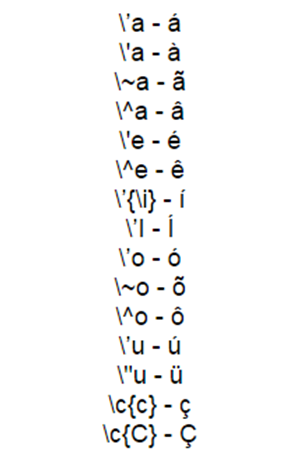
\includegraphics[scale=1.0]{imagens/USPSC-AcentuacaoLaTeX.png} \\
	%Fonte: \citeonline{comandos}
	Fonte: \citefonte{comandos}

\end{figure}

\end{anexosenv}


\end{document}
